
%% jan. 4, 2011  items to fix:
%% notation for math and reference to images.
%% how include eps figures.
%% make all the little figures (search for eps) in a common, nice matlab way for the
%% example filtering operations.

%\setcounter{chapter}{22}
\chapter{Temporal Filters}
\label{chapter:temporal_filters}

%\section{Temporal convolutional filters}


\section{Introduction}

Although adding time might seem like a trivial extension from two-dimensional (2D) signals to three-dimensional (3D) signals, and in many aspects it is, there are some properties of how the world behaves that make sequences seem different from arbitrary 3D signals. In 2D images most objects are bounded, occupying compact and well defined image regions. However, in sequences, objects do not appear and disappear instantaneously unless they get occluded behind other objects or enter or exit the scene through doors or the image boundaries. So, the behavior of an object across time $t$ is very different than its behavior across space $n,m$. In time, objects move and deform defining continuous trajectories that have no beginning and never end. 


\section{Modeling Sequences}
\label{sect:modelingSequences}

Sequences will be represented as functions $\img (x,y,t)$, where $x,y$ are the spatial coordinates and $t$ is time. As before, when processing sequences we will work with the discretized version that we will represent as $\img \left[n,m,t \right]$, where $n,m$ are the pixel indices and $t$ is the frame number. Discrete sequences will be bounded in space and time, and can be stored as arrays of size $N \times M \times P$.


\Fig{\ref{fig:motion}} illustrates this with one sequence, as shown in \fig{\ref{fig:motion}}{a}. This sequence has 90 frames and shows people on the street walking parallel to the camera plane and at different distances from the camera. \Fig{\ref{fig:motion}}{b} shows the space-time array $\img \left[n,m,t \right]$. When we look at a picture we are a looking at a 2D section, $t=constant$, of this cube. But it is interesting to look at sections along other orientations.  Figures \ref{fig:motion}(c-d) show sections for $m=constant$ and $n=constant$, respectively. Although they are also 2D images, their structure looks very different from the images we are used to seeing. \Fig{\ref{fig:motion}}{c} shows a horizontal section that is parallel to the direction of motion of the people walking. Here we see straight bands with different orientations. The bands appear to occlude each other. Each band corresponds to one person and its orientation is given by the speed and the direction of motion. \Fig{\ref{fig:motion}}{d} looks like a photo-finish picture like the ones used in sporting races. In both figures \ref{fig:motion}(c and d), static objects appear as vertical stripes in \fig{\ref{fig:motion}}{b}, and horizontal stripes in \fig{\ref{fig:motion}}{d}. 


\begin{figure}
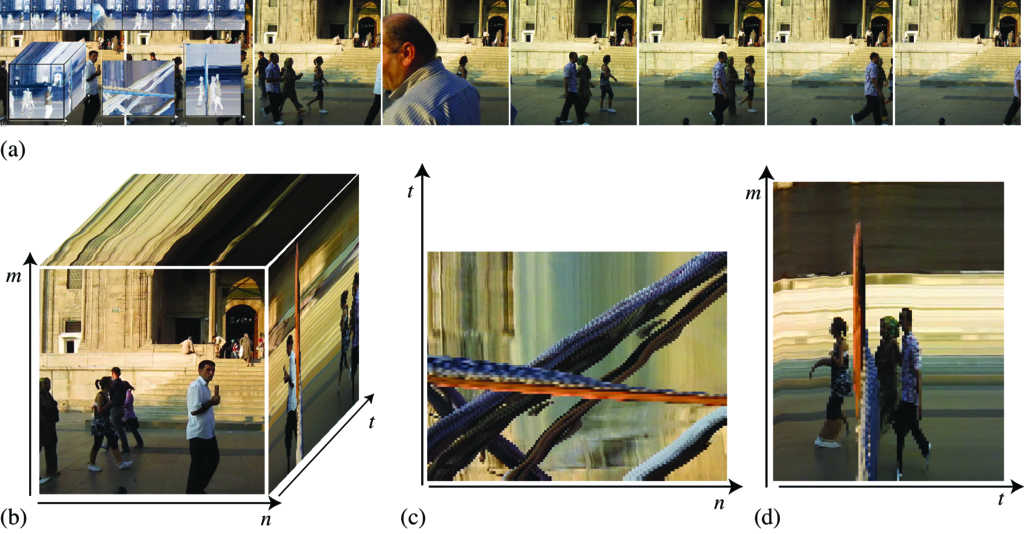
\includegraphics[width=1\linewidth]{figures/temporal_filters/motion_illustration.eps}
\caption{(a) Eight frames from a sequence with people walking. The frames are shown at regular time intervals. The full sequence had 90 frames (corresponding to 3 s of video). (b) Space-time array, $\img \left[n,m,t \right]$ of size $128 \times 128 \times 90$. (c) Section for $m=50$. (d) Section for $n=75$. Static objects appear as straight lines.} 
\label{fig:motion}
\end{figure}


One special sequence is when the image has a global motion with constant velocity $(v_x,v_y)$. In such a case we can write:
\begin{equation}
\img (x,y,t) = \img_0 (x-v_x t,y-v_y t)
\label{eq:globaly_moving_image}
\end{equation}
where $\img_0(x,y)= \img (x,y,0)$ is the image being translated, and $v_x$ and $v_y$ are constants. At time $t$ the image $\img_0(x,y)$ is translated by the vector $(v_x t,v_y t)$ as described by \eqn{\ref{eq:globaly_moving_image}}. The pixel value at location $(x=0, y=0)$ at time $t=0$ will appear at time $T$ in location $(x=v_x T, y=v_y T)$.
This is what we see in \fig{\ref{fig:motion}}{c} where the bands are created by moving pixels.

We use continuous values for $x$, $y$, and $t$, and continuous images, $\img_0(x,y)$,  because it allows us to deal with any velocity values. This function also assumes that the brightness of the pixels does not change while the scene is moving ({\bf constant brightness assumption}). \marginnote{The constant brightness assumption is the initial hypothesis of most motion estimation algorithms. We will devote multiple chapters in part \ref{part:understanding_geometry} to study motion in depth.}
\index{Constant brightness assumption}


In general, sequences will be more complex, but the properties of a globally moving image are helpful to understand local properties in sequences. We can also write models for more complex sequences. For instance, a sequence containing a moving object over a static background can be written as: 
\begin{equation}
\img (x,y,t) = b(x,y) (1-m(x-v_xt,y-v_yt)) + o(x-v_xt,y-v_yt) m(x-v_x t,y-v_y t)
\end{equation}
where $b(x,y)$ is the static background image, $o(x,y)$ is the object image moving with speed $(v_x,v_y)$, and $m(x,y)$ is a binary mask that moves with the object and that models the fact that the object occludes the background. 

\section{Modeling Sequences in the Fourier Domain}
\label{section:Modeling_sequences_in_the_Fourier_domain}

The Fourier transform (FT) of a globally moving image, \eqn{\ref{eq:globaly_moving_image}}, is (using the shift property):
\begin{equation}
\capitalimg (w_x,w_y,w_t) = \capitalimg_0 (w_x, w_y) \delta (w_t + v_x w_x + v_y w_y)
\end{equation}
The continuous FT of the sequence is equal to the product of the 2D FT of the static image $\img_0(x,y)$ and a delta wall. To better understand this function let's look at a simple example on only one spatial dimension, as shown in \fig{\ref{fig:mov_pulse_012}}. 

\begin{figure}[t]
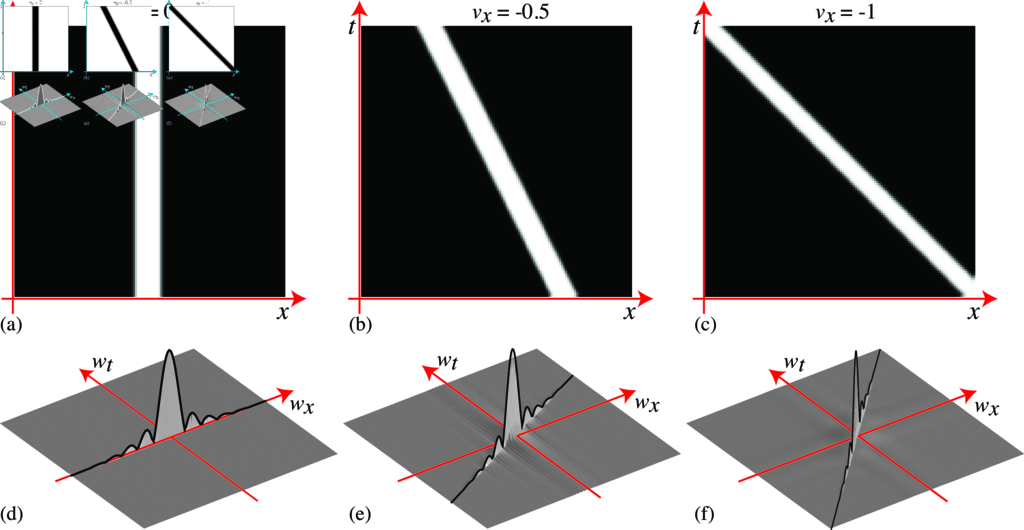
\includegraphics[width=1\linewidth]{figures/temporal_filters/mov_pulse_012.eps}
\caption{(a) A sequence with one spatial dimension showing a static rectangular pulse. (b) The rectangular pulse moves toward the left at speed $v=-0.5$, and (c) toward the left, $v=-1$. As we work with discretized signals, speed units are in pixels per frame.} 
\label{fig:mov_pulse_012}
\end{figure}

\Fig{\ref{fig:mov_pulse_012}} shows the FT for a sequence with one spatial dimension, $\img(x,t)$, that contains a blurry rectangular pulse moving at three different speeds toward the left. \Fig{\ref{fig:mov_pulse_012}}{a} shows a sequence when the pulse is static and \fig{\ref{fig:mov_pulse_012}}{d} shows its FT.  Across the spatial frequency $w_x$, the FT is approximately a sinc function.
Across the temporal frequency $w_t$, as the signal is constant, its FT is a delta function.  Therefore the FT is a sinc function contained inside a delta wall in the line $w_t=0$. \Fig{\ref{fig:mov_pulse_012}}{b} shows the same rectangular pulse moving towards the left, $v_x=0.5$. \Fig{\ref{fig:mov_pulse_012}}{e} shows the sinc function but skewed a long the frequency line $w_t+0.5w_x=0$. Note that this is not a rotation of the sinc function from \fig{\ref{fig:mov_pulse_012}}{d} as the locations of the zeros lie at the same $w_x$ locations. \Fig{\ref{fig:mov_pulse_012}}{c} shows the pulse moving at a faster speed resulting in a larger skewing of its FT, \fig{\ref{fig:mov_pulse_012}}{f}.

\marginnote{The {\bf sinc function} is the FT of a box kernel. In the continuous domain, the sinc function has the form:
\begin{equation*}
    \text{sinc}(x) = \frac{\sin (\pi x)}{\pi x}
\end{equation*}
This function has its maximum at $x=0$ and then has decreasing oscillations.
\\[6pt]
\centerline{
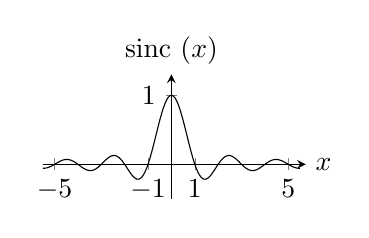
\begin{tikzpicture}
\begin{axis} [width=140pt,height=90pt,
	axis x line=middle, 
	axis y line=middle, 
	tick align=center,
	every axis x label/.style={at={(current axis.right of origin)},anchor=west},
	every axis y label/.style={at={(current axis.above origin)}, anchor=north east,above=0mm},
	xmin=-5.5, xmax=5.75,
	xtick={-5,-1,0,1,5},
    %xticklabels = {$-2\pi$, $0$, $2\pi$},
	xlabel=$x$,
	ymin=-.5, ymax=1.3,
	ytick={0,1},
	ylabel={sinc $\left(x\right)$}]
\addplot[domain=-5.5:5.5,samples=102,samples y=0] ({x}, {sin(deg(pi*x)) / (pi*x)}); 
%\addplot[domain=-14:14,samples=102,samples y=0,draw=blue] ({x}, 1/abs(x)}); 
\end{axis} 
\end{tikzpicture}
}
\\[6pt]
We will discuss this further in \sect{\ref{sec:aliasing:ideal_reconstruction}}.
} 
%We let to the reader the work of computing its FT and visualizing the effect of the mask in the Fourier domain.



\section{Temporal Filters}

Linear spatiotemporal filters can be written as spatiotemporal convolutions between the input sequence and a convolutional kernel (impulse response). 
\index{Filter!Spatiotemporal}
Discrete spatiotemporal filters have an impulse response $h \left[n,m,t \right]$, where the independent variables $n$, $m$, and $t$ are discrete and only take on integer values. The extension from 2D filter to spatiotemporal filters does not has any additional complications. We can also classify filters as low-pass, high-pass, and so on. But in the case of time, there is another attribute used to characterize filters, namely {\bf causality}: 
\begin{itemize} 
\item Causal filters. 
\index{Filter!Causal}
These are filters with output variations that only depend of the past values of the input. This puts the following constraint: $h \left[n,m,t \right]=0$ for all $t<0$. This means that if the input is an impulse at $t=0$, the output will only have non-zero values for $t>0$. If this condition is satisfied, then the filter output will only depend on the input's past for all possible inputs. 
\item Noncausal filters. When the output has dependency on future inputs.
\item Anticausal filters. 
\index{Filter!Anticausal}
This is the opposite, when the output only depends on the future: $h \left[n,m,t \right]=0$ for all $t>0$.
\end{itemize}
Many filters are noncausal and have both causal and anticausal components (e.g., a Gaussian filter). Note that noncausal filters can not be implemented in practice and, therefore, any filter with an anticausal component will have to be approximated by a purely causal filter by bounding the temporal support and shifting in time the impulse response. 

In this chapter, we have written all the filters as convolutions. However, some filters are better described as difference equations (this is specially important in time). An example of a difference equation is:
\begin{equation}
\imgout \left[n,m,t \right] = \imgin \left[n,m,t \right] + \alpha \, \imgout \left[n,m,t-1 \right]
\end{equation}
where the output $\imgout$ at time $t$ depends on the input at time $t$ and the output at the previous time instant $t-1$ multiplied by a constant $\alpha$. We can easily evaluate the impulse response, $h \left[n,m,t \right]$, of such a filter by replacing $\imgin \left[n,m,t \right]$ with an impulse, $\delta \left[n,m,t \right]$. 
\marginnote{Remember that $\delta \left[n,m,t \right]$ is 1 for $n=0,m=0,t=0$, and 0 everywhere else.}[-.2in]
The impulse response is:
\begin{equation}
h \left[n,m,t \right] = \alpha^t  \delta \left[n,m \right] u \left[t \right]
\end{equation}
where $u\left[t \right]$, called the {\bf Heaviside step} function, is:
\begin{equation}
u \left[t \right] = \begin{cases}
    0     & \quad \text{if }  t <0 \\
    1     & \quad \text{otherwise }\\
\end{cases}
\end{equation}
\marginnote{The Heaviside step function, $u \left[t\right]$, is an infinite length function with the form
\\[6pt]
\centerline{
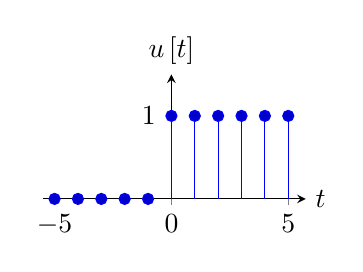
\begin{tikzpicture}
\begin{axis} [width=140pt,height=90pt,
	axis x line=bottom, 
	axis y line=middle, 
	tick align=center,
	every axis x label/.style={at={(current axis.right of origin)},anchor=west},
	every axis y label/.style={at={(current axis.above origin)}, anchor=north east,above=0mm},
	xmin=-5.5, xmax=5.75,
	%xtick={-3,...,6},
	xlabel=$t$,
	ymin=0, ymax=1.5,
	ytick={0,1},
	ylabel={$u \left[t\right]$}]
\addplot+[ycomb] plot coordinates {(-5,0) (-4,0) (-3,0) (-2,0) (-1,0) (0,1) (1,1) (2,1) (3,1) (4,1) (5,1)};
\end{axis} 
\end{tikzpicture}
}
}[-0.6in]

Most filters described by differences equations have an impulse response with infinite support. They are called Infinite Impulse Response (IIR) filters.
\index{Filter!Infinite impulse response}
IIR filters can be further classified as stable and unstable. {\bf Stable} are the ones that given a bounded input, $| \imgin \left[n,m,t \right] |<A$, produce a bounded output, $| \imgout \left[n,m,t \right] | <B$. For this to happen, the impulse response has to be bounded. In {\bf unstable} filters, the amplitude of the impulse response diverges to infinity. In the previous example, the filter is stable if and only if $| \alpha | < 1$. 
\index{Filter!Stability}


Let's now describe some spatiotemporal filters. 


\subsection{Spatiotemporal Gaussian}

As with the spatial case, we can define the same low-pass filters in the spatiotemporal domain: the box filter, triangular filters, and so on.  As an example, let's focus on the Gaussian filter. The spatiotemporal Gaussian is a simple extension of the spatial Gaussian filter in section~\ref{sec:spt_gaussian}:
\index{Filter!Spatiotemporal Gaussian}
\begin{equation}
g(x,y,t; \sigma_x,\sigma_t) = \frac{1}{(2 \pi)^{3/2} \sigma_x^2\sigma_t} \exp{-\frac{x^2 +
   y^2}{2 \sigma_x^2}} \exp{-\frac{t^2}{2 \sigma_t^2}}
\label{eq:gauss3dcont}
\end{equation}
where $\sigma_x$ is the width of the Gaussian along the two spatial dimensions, and $\sigma_t$ is the width on the temporal domain. As the units for $t$ and $x,y$ are unrelated, it does not make sense to set all the $\sigma$s to have the same value. 

We can discretize the continuous Gaussian by taking samples and building a 3D convolutional kernel. We can also use the binomial approximation. The 3D Gaussian is separable so it can be implemented efficiently as a convolutional cascade of three one-dimensional (1D) kernels. \Fig{\ref{fig:seq_filtered_kernel}}{a} shows a spatiotemporal Gaussian. The temporal Gaussian is a noncausal filter, therefore it is not physically realizable. This is not a problem when processing a video stored in memory. However, if we are processing a streamed video, we will have to bound and shift the filter to make it causal, which will result in a delay in the output. 


\begin{figure}[t]
\includegraphics[width=1\linewidth]{figures/temporal_filters/seq_filtered_kernel.eps}
\caption{(a) Spatiotemporal Gaussian with $\sigma=1$ and $\sigma_t=4$.  (b) Same Gaussian parameters but skewed by the velocity vector $v_x=-1, v_y=0$ pixels/frame, and (c) $v_x=1, v_y=0$ pixel/frame.} 
\label{fig:seq_filtered_kernel}
\end{figure}

\Fig{\ref{fig:sec_filtered_blur}}{a} shows one sequence and \fig{\ref{fig:sec_filtered_blur}}{b} shows the sequence filtered with the Gaussian from \fig{\ref{fig:seq_filtered_kernel}}{a}. This Gaussian has a small spatial width, $\sigma=1$, and a large temporal width, $\sigma_t=4$ so the sequence is strongly blurred across time. The moving objects show motion blur and are strongly affected by the temporal blur, while the static background is only affected by the spatial width of the Gaussian.


\begin{figure}[t]
\includegraphics[width=1\linewidth]{figures/temporal_filters/seq_filtered_blur.eps}
\caption{(a) One frame from the input sequence and the space-time section (on top). (b) Output when convolving the Gaussian from \fig{\ref{fig:seq_filtered_kernel}}{a}. (c) Output of the convolution with \fig{\ref{fig:seq_filtered_kernel}}{b}. (d) Output of the convolution with \fig{\ref{fig:seq_filtered_kernel}}{c}.} 
\label{fig:sec_filtered_blur}
\end{figure}

How could we create a filter that keeps sharp objects that move at some velocity $(v_x,v_y)$ while blurring the rest? \Fig{\ref{fig:sec_filtered_blur}}{c} shows the desired output of such a filter. The bottom image shows one frame for a sequence filtered with a kernel that keeps sharp objects moving left at 1 pixel/frame while blurring the rest. This filter can be obtained by skewing the Gaussian:
\begin{equation}
g_{v_x,v_y}(x,y,t) = g(x - v_xt,y - v_yt, t) 
\end{equation}
%where $g_{v_x,v_y}(x,y,t)$ is a skewed gaussian a long the space-time direction $(v_x,v_y,1)$. 
This directional blur is not a rotation of the original Gaussian as the change of variables is not unitary, but the same effect could be obtained with a rotation. \Fig{\ref{fig:sec_filtered_blur}}{c} shows the effect when $v_x=-1, v_y=0$. The Gaussian is shown in \fig{\ref{fig:seq_filtered_kernel}}{b}. The space-time section shows how the sequence is blurred everywhere except one oriented bad corresponding to the person walking left. \Fig{\ref{fig:sec_filtered_blur}}{d} shows the effect when $v_x=1, v_y=0$. The output of this filter looks as if the camera was tracking one of the objects while the shutter was open, producing a blurry image of all the other objects.


\subsection{Temporal Derivatives}


Spatial derivatives are useful to find regions of image variation such as object boundaries. Temporal derivatives can be used to locate moving objects. We can approximate a temporal derivative for discrete signals as the difference:
\begin{equation}
\img \left[m,n,t\right] - \img \left[m,n,t-1\right] 
\end{equation}

\marginnote{When implementing temporal filters it is important to use causal filters. A causal filter depends only on the present and past input samples.}

As in the spatial case, it is useful to compute temporal derivatives of spatiotemporal Gaussians:
\begin{equation}
\frac{\partial g}{\partial t} = \frac{-t}{\sigma_t^2} g(x,y,t)
\end{equation}
where $g(x,y,t)$ is the Gaussian as written in \eqn{\ref{eq:gauss3dcont}}. We can compute the spatiotemporal gradient of a Gaussian:
\begin{eqnarray}
\nabla  g &=& \left( g_x(x,y,t), \, g_y(x,y,t), \, g_t(x,y,t) \right) \nonumber \\
 &=&  \left(-x/\sigma^2, -y/\sigma^2, -t/\sigma_t^2 \right) g(x,y,t)
 \label{eq:spt_gradient_gaussian}
\end{eqnarray}
We can use the analytic form of the spatiotemporal Gaussian derivatives from \eqn{\ref{eq:spt_gradient_gaussian}} to discretize the filter, by taking samples at discrete locations in space and time, and use the resulting discrete spatiotemporal kernel to filter an input discrete sequence. These filters can be used for many applications. Let's look at one practical example: What should we do if we want to remove from a sequence the objects moving at a particular velocity? 

To answer that question, we will first assume the sequence contains a single object moving at a constant velocity. We will then compute the  derivatives along $x$, $y$, and $t$ of the sequence and we will find out what particular linear combination of those derivatives makes the output go to zero only when the input sequence moves at a target velocity.

In the case of an image, $\img_0 (x,y)$, that moves with velocity $(v_x, v_y)$, the sequence is 
\begin{equation}
\img (x,y,t) = \img_0 (x-v_xt,y-v_yt)
\end{equation}
We can compute the temporal derivative of $\img (x,y,t)$ as:
\begin{equation}
\frac{\partial \img}{\partial t} = \frac{\partial \img_0}{\partial t} = -v_x \frac{\partial \img_0}{\partial x} - v_y \frac{\partial \img_0}{\partial y}
\label{eq:brightnessconstancy}
\end{equation}
This result is interesting because it shows that for a moving image there is a relationship between the temporal derivative of the sequence and the spatial derivatives a long the direction of motion. We can use this relationship to find a linear combination of the temporal and spatial derivatives so that the output is zero. 

In fact, if we compute the gradient of the Gaussian along the vector $\left[1,v_x,v_y\right]$:
\begin{equation}
h(x,y,t;v_x,v_y) = g_t+v_xg_x+v_yg_y = \nabla  g \left( 1,v_x,v_y \right)^\transpose
\label{eq:spt_nulling_filter}
\end{equation}
we get a kernel $h(x,y,t;v_x,v_y)$ that we can use as a spatiotemporal filter that will do exactly what we were looking for. Indeed, if we convolve it with the input sequence $\img_0 (x-v_xt,y-v_yt)$ we get a zero output (using equation [\ref{eq:brightnessconstancy}]):
\begin{eqnarray}
\img_0 (x-v_xt,y-v_yt) \circ h &=& \img_0 (x-v_xt,y-v_yt) \circ \left(  g_t+v_xg_x+v_yg_y \right) \nonumber \\
&=& \left( \frac{\partial \img_0}{\partial t} + v_x \frac{\partial \img_0}{\partial x} + v_y \frac{\partial \img_0}{\partial y} \right) \circ g \nonumber \\
&=& 0 \nonumber
\end{eqnarray}

The filter $h$ from \eqn{\ref{eq:spt_nulling_filter}} is shown in \fig{\ref{fig:gaussian_seq}}. As this filter is 3D we show as a sequence for different velocities. Each row in the figure corresponds to one particular velocity $v_x,v_y$. In the example shown in  \fig{\ref{fig:gaussian_seq}}{a} the Gaussian has a width of $\sigma^2=\sigma_t^2=1.5$, and has been discretized as a 3D array of size $7 \times 7 \times 7$. Figures \ref{fig:gaussian_seq}(b,c and d)  show the filter $h$ for different velocities: $(v_x,v_y) =$ $(0,0)$, $(1,0)$ and $(-1,0)$. 

\begin{figure}
\includegraphics[width=1\linewidth]{figures/temporal_filters/gaussians_xyt_seq.eps}
\caption{Visualization of the space-time Gaussian. The Gaussian has a width of $\sigma^2=\sigma_t^2=1.5$, and has been discretized as a 3D array of size $7 \times 7 \times 7$. Images along each row show the seven frames of each spatiotemporal discrete Gaussian. (a)  Gaussian. (b) The partial derivative of the Gaussian with respect to $t$. (c) Derivative along $v=(1,0)$ pixels/frame. (d) $v=(-1,0)$ pixels/frame.} 
\label{fig:gaussian_seq}
\end{figure}

\Fig{\ref{fig:gaussian_xyt_section}} shows a different visualization of the same filter $h$ from \eqn{\ref{eq:spt_nulling_filter}}. Each image in \fig{\ref{fig:gaussian_xyt_section}}
shows a space-time section of the same spatiotemporal Gaussian derivatives as the ones shown in \fig{\ref{fig:gaussian_seq}}. Both visualizations are equivalent and help to understand how the filter works.


\begin{figure}
\includegraphics[width=1\linewidth]{figures/temporal_filters/gaussians_xyt_section.eps}
\caption{Spatiotemporal Gaussian $g\left[ n,t \right]$ and derivatives. (a) Gaussian with $\sigma^2=1.5$. (b) Partial derivative with respect to $t$. c) Partial derivative along $(1,-1)$. (d) Partial derivative along $(1,1)$. The result of adding values along the green line is zero.} 
\label{fig:gaussian_xyt_section}
\end{figure}

%
%This is because we are computing spatio-temporal derivatives a long the direction of motion, so any object moving at that particular speed will be a constant a long that direction and its derivative will be zero. Fig.~\ref{fig:gaussian_xyt_section} shows a discrete spatio-temporal gaussian and temporal derivatives. Fig.~\ref{fig:gaussian_xyt_section}.a shows the gaussian across one spatial dimension and time. Fig.~\ref{fig:gaussian_xyt_section}.b is the temporal derivative, Fig.~\ref{fig:gaussian_xyt_section}.c shows the discretized gaussian gradient $g_t \left[n,t \right]+v_x g_x \left[ n,t \right]$ with $v_x=-1$ and Fig.~\ref{fig:gaussian_xyt_section}.d with $v_x=1$.


Such a filter $h$ will cancel any objects moving at the velocity $(v_x,v_y)$. By using different filters, each one computing derivatives a long different space-time orientations, we can create output sequences where specific objects disappear, as shown in \fig{\ref{fig:tunedfilter}}. This filter is called a {\bf nulling filter} \cite{Darrell93}.
\index{Filter!Nulling filter}

\begin{figure}
\includegraphics[width=1\linewidth]{figures/temporal_filters/seq_filtered_der.eps}
\caption{(a) Input sequence. (b) Output to $h$ with $v_x=v_y=0$. (c) $v_x=1$ pixels/frame. (d) $v_x=-1$ pixel/frame.} 
\label{fig:tunedfilter}
\end{figure}


Note that despite that we assumed that the sequence contained a single moving object when deriving the formulation for the nulling filter, the filter also works in sequences with multiple objects moving a different speeds as shown in \fig{\ref{fig:tunedfilter}}. This is because the operations are local (the kernel $h$ has a small size) and the behavior will be correct if in a local image patch there is only one velocity present. In fact, it is easy to show that the method will also work if the sequence is a sum of several moving transparent layers. 


\section{Concluding Remarks}
%\reviewcomment{To be written.}

In this chapter we have discussed different types of spatiotemporal filters used to analyze video. However, we have not presented how these filters can be used to estimate useful quantities such as velocity. We will devote several chapters in part \ref{part:understanding_motion} to motion estimation. 

